\documentclass [12pt]{article}

\usepackage{amsmath, amsthm, amssymb, amsfonts}
\usepackage{mathptmx}
\usepackage{thmtools}
\usepackage{graphicx}
\usepackage{setspace}
\usepackage{float}
\usepackage{hyperref}
\usepackage[utf8]{inputenc}
\usepackage[english]{babel}
\usepackage{framed}
\usepackage[dvipsnames]{xcolor}
\usepackage{tcolorbox}
\usepackage{ mathrsfs }
\usepackage{tfrupee}
\usepackage{times}
\usepackage{booktabs}
\usepackage{rotating} % For rotating the table
\usepackage{caption}  % For adding captions to tables
\usepackage{relsize}
\usepackage{multicol}
\usepackage{lipsum} % For generating dummy text
\usepackage{threeparttable}
\usepackage{csquotes} 
\usepackage{array}
\usepackage{pifont}
\usepackage{tikz}
\usetikzlibrary{positioning, shapes.geometric, arrows.meta}
\usepackage[toc]{appendix}
\colorlet{LightGray}{White!90!Periwinkle}
\colorlet{LightOrange}{Orange!15}
\colorlet{LightGreen}{Green!15}
\usepackage[left=1in, right=1in, top=1in, bottom=1in]{geometry}
\usepackage[backend=biber, style=apa]{biblatex}

\addbibresource{ref.bib}



\newcommand{\HRule}[1]{\rule{\linewidth}{#1}}


\setstretch{1.2}
\geometry{
    textheight=9in,
    textwidth=5.5in,
    top=1in,
    headheight=12pt,
    headsep=25pt,
    footskip=30pt
}

%\DTMlangsetup{showdayofmonth=false} % to hide day of the month

\begin{document}

\begin{titlepage}
    \centering
    \vspace*{1cm}

    \LARGE \textbf{Assessing the Poverty Alleviating Effects of MSME in India}\\[0.5cm]

    \Large{An Undergraduate Thesis}\\[2cm]

    \normalsize Submitted in fulfillment of the requirements for the degree of\\
    Bachelors of Science in Economics\\[2cm]

    \normalsize at\\
    Gokhale Institute of Politics and Economics\\
    (University u/s 3 of UGC Act, 1956)\\[1cm]

    \normalsize by\\
    Mr.\ Ishan Deodhar\\[0.5cm]
    
    \normalsize Under guidance of\\
    Mr.\ Balu Pawde\\[1cm]

    \vspace*{3cm}

    Gokhale Institute of Politics and Economics, Pune\\
    March, 2024\\[2cm]

\end{titlepage}

\newpage
\pagenumbering{gobble}
\section*{Declaration}

\normalsize
I, Mr.\ Ishan Deodhar, hereby declare that this dissertation is the result of my study under the guidance and supervision of Mr.\ Balu Pawde from the Gokhale Institute of Politics and Economics, Pune. This work has not previously been used to award any degree, diploma, or certificate from this Institute or any other University. I have properly acknowledged all sources used in the preparation of this dissertation.
\vspace{16cm}

Mr.\ Ishan Deodhar

\today

\newpage
\section*{Certificate}

\normalsize
This is to certify that the dissertation presented is an original work by Mr.\ Ishan Deodhar, registered under BECO21230, and was produced under my guidance and supervision. The research results in this project report have not previously served as the basis for the award of any degree, diploma, or certificate from this institute or any other educational institution.
\vspace{16cm}

Mr.\ Balu Pawde

Assistant Professor, GIPE

\today

\newpage
\section*{Acknowledgment}

\normalsize
First and foremost, I express my sincere appreciation to Mr.\ Balu Pawde, who has been a consistent source of assistance and guidance throughout my academic journey. I am genuinely grateful for his valuable wisdom and expertise, which have greatly influenced and shaped my ideas. I extend my gratitude to Mr.\ Ayush Patel for his critical feedback and assistance with data analysis and computational methodologies. My sincere thanks go to Ms.\ Santoshi Rajguru for her essential guidance in comprehending the ASI data. I want to thank my friends and colleagues at Gokhale Institute for being a constant source of encouragement and support. I would like to extend special thanks to Ms.\ Jayati Sharma for her thorough review of my code. I am deeply grateful to Ms.\ Anuja Baldota, Ms.\ Srushti Bhambhere and Ms.\ Chandrima Dey for their unwavering support and for ensuring I maintained my sanity throughout this process.

\newpage

\tableofcontents
\newpage

\newgeometry{top=2cm, bottom = 2.2cm, left = 2.5cm, right = 2.5cm}
\pagenumbering{arabic}
\section{Introduction}
\paragraph{} Poverty alleviation has been at the centre of the Indian development agenda. At independence, poverty was sought to be alleviated through rapid industrialisation and large public works projects, by bolstering employment \parencite{balakrishnan_indias_economy}. Then, in the 1970s, poverty alleviation was the main objective of the fifth five-year plan \parencite{kapila_indian_economy}. The 1970s also saw the emergence of poverty alleviation schemes like IRDP (Integrated Rural Development Program), where self-employment was encouraged and assets in the form of livestock were distributed. Poverty alleviation remained a key objective of many succeeding five-year plans of the Government of India. The Public Distribution System (PDS) has been instrumental in alleviating poverty in India. \textcite{kumar2015public} explain the role of India's triumph in alleviating poverty through PDS, and assert the importance of PDS on the nutrition of the Below Poverty Line (BPL) children. The National Rural Employment Guarantee Act (NREGA), introduced in 2005, has played a crucial role in poverty alleviation. \textcite{klonner2022welfare} note the effects f NREGA on poverty reduction, while \textcite{Niehaus&Sukhtanker2013} criticise the inefficiencies and corruption in the implementation of NREGA. Poverty alleviation is the first of the Sustainable Development Goals (SGD) to which India has committed. Official estimates suggest that the incidence of poverty headcount has declined from 37\% in 2004-05 to 21\% in 2011-12 \autocite{planningcommission2013}.

\text The current ministry of Micro, Small and Medium enterprises (MSME) can find its roots in the `Small Scale Industries Board' (SSI), established in 1955. In 1999, SSI and the Ministry of Agro and Rural Industries (ARI) were created by the Government of India. In 2006, both of these ministries were merged to form the current Ministry of MSME.  \textcite{amutha2022role} concludes that MSME are the primary
source of employment, production, exports, and GDP growth in India.
 ``This sector employs an estimated 59.7 million persons spread over 31 million enterprises. It is estimated that in terms of value, MSME sector accounts for about 45\% of the manufacturing output and around 40\% of the total export of the country'' \parencite[739]{purakala2020role}. MSME contribute 36\% to the country's manufacturing sector's output and 29\% of the country's GVA \parencite{MSME2023}. Certainly, MSME constitute a pivotal sector within the Indian economy.

\textcite{singh1999role} defines the relationship between employment and poverty reduction could be attained on three conditions: (i) the overall growth rate of labour must be able to absorb new workers with high levels of productivity, (ii) job creation must produce an equitable job distribution between the poor and non-poor, and (iii) the jobs created must have a wage standard or at least a livable, satisfactory wage. \textcite{islam2004nexus} asserts that when a high level of economic growth leads to increased production capacity and productivity, the poor have an opportunity to be absorbed into the various productive sectors that can generate higher incomes. Through this process, each labourer absorbed into these sectors would positively affect poverty alleviation. Thus, combining \textcite{islam2004nexus}, \textcite{singh1999role}, \textcite{MSME2023}, and \textcite{purakala2020role} MSME may lead to poverty alleviation in India. This study aims to find this empirically. 
\newpage
\restoregeometry
\section{Literature Review}             

\paragraph{} \textcite{green2006finance},  analyse the connection between financial sector development and the growth of micro and small enterprises (MSE) for poverty reduction in developing countries, highlighting the need for policies that improve access to financial services for MSE. It points out the transition from traditional credit methods to more holistic financial services, emphasizing their importance in poverty alleviation. \textcite{mbuyisaetal} conduct a comprehensive review of literature and find that ICT enables better communication and information sharing, and increases the efficiency and market reach of small and medium enterprises (SME) which in turn contribute to income and employment generation, and aid in poverty reduction. \textcite{kersten2017small} review systemic literature on SME financing and also conduct a multivariate meta-analysis of SME finance programs in Low and Middle-Income Countries (LMICs), to evaluate the impact on employment, firm performance, and economic development. \textcite{kersten2017small} find a positive, significant effect of SME finance on capital investment, firm performance, and employment, however, the impact on profitability and wages is found to be insignificant. \textcite{kersten2017small} conclude that while SME finance positively impacts the firm’s performance, its effects on broader economic development remain unclear.

\textcite{vandenberg2006poverty} explores the significance of small enterprises in alleviating poverty. The study highlights crucial elements like the necessity for supportive policies, accessible financing options, appropriate training, and infrastructure development for small enterprises to alleviate poverty. Key challenges are addressed, such as evolving from micro to medium-sized enterprises, evaluating SED's (Small Enterprise Development) influence on poverty reduction, and finding a balance between market autonomy and regulatory intervention. Furthermore, the research delves into the International Labour Organization's (ILO) strategies and their alignment with the Millennium Development Goals.

\textcite{harvie2003contribution} found that growth of SME in East Asian Countries\footnote{Cambodia, China, Hong Kong, Indonesia, Korea, Laos, Malaysia, Mongolia, Myanmar, Philippines, Singapore, Taiwan, Thailand, and Vietnam} improved the living standards of the poor. \textcite{MAKSIMOV2017244} find that female ownership, government contract, and export of SME increases Organisational efficiency and that increases wages, and that in return reduces poverty in Least Developed Countries\footnote{Afghanistan, Nepal, Mali, Mozambique, Senegal, Yemen and Zambia}. \textcite{wibiseno2021influence} find that labour, business capital, and technology simultaneously have a significant impact on the income of MSME. The findings suggest that improvements in production technology can enhance the efficiency of MSME, leading to increased income levels, aligning with \textcite{MAKSIMOV2017244}. \textcite{Beck2003SMEGrowth} analyse relationship between the size of the SME sector and economic growth and poverty alleviation in 75 countries.  They find a positive association between SME size and economic growth, but this correlation weakens upon controlling for simultaneity bias, indicating that SME are common in successful economies and may not causally impact growth. \textcite{Beck2003SMEGrowth} do not find any significant relationship between SME and poverty alleviation. \textcite{abisuga2020smes} conclude that supporting SME growth and addressing their challenges via policy can significantly enhance employment generation and poverty alleviation in Sub-Saharan Africa. \textcite{Agupusi2007} examines the role of MSME in poverty alleviation in Alexandra, South Africa. The study highlights that there is an increased participation of the private sector and local communities in small business development since 1994. \textcite{Agupusi2007} critically assesses government and private sector initiatives supporting small business development for poverty alleviation and notes that small businesses, especially in semi-formal and informal sectors, are not effectively contributing to poverty reduction due to various constraints, the paper argues that positive interaction between development agencies and small businesses, especially in informal and semi-formal sectors, could significantly alleviate poverty and contribute to overall transformation in Alexandra. 

\textcite{nursini2020msmes} computes direct and indirect effects of MSE and SME on Poverty Headcount index, Poverty Gap index, and Poverty Severity index in Indonesia, and finds that an increase in MSME output has a negative effect on all three indicators. Nursini also finds the effects of MSE to have a larger poverty reduction effect than SME. \textcite{yuniar2015development} using case-study methodology posits that Baitul Maal Wat Tamwil (BMT), a micro-finance institution,  aids poverty alleviation by providing financial support and business mentoring to MSME. \textcite{asikhia2016smes} looks at the role of Human Resources, Technology, Innovation, Strategy, Unit cost Economies, and Organisational Infrastructure of 518 SME in Nigeria on Wealth Creation, Wealth Distribution and Wealth Motivation, and effect of these on Poverty Alleviation. \textcite{asikhia2016smes} finds that  15\% of wealth created that contributed to alleviating poverty was traceable  to  SME. This claim is supported by \textcite{kowo2019role}, they find that SME contribute towards employment generation in Nigeria and reduce poverty significantly.
\textcite{ali2014role} find output of SME have a negative effect on poverty headcount ratio in Pakistan. \textcite{vijayakumar2013empirical} explores role of SME on Sri Lanka's economic growth and poverty reduction, and finds that SME do not have a significant relationship with poverty or economic growth, in line with \textcite{manzoor2019role}.  \textcite{begum2015employment} note that SME spread across various regions (clusters) of Bangladesh are creating jobs and income for their workforce while also manufacturing products that may be substituted for imports. \textcite{BAUCHET2013288} compare the impact of microcredit and SME finance on employment and poverty reduction in Bangladesh. They find that SME employees generally have higher educational levels, professional skills, and live in less impoverished conditions compared to microcredit users. Their research suggests that SME finance isn't as effective in job creation for the demographic typically served by microcredit. They conclude that microcredit and SME finance should be seen as complementary strategies rather than interchangeable solutions in the context of alleviating poverty. 
\textcite{manzoor2019role} find a positive effect of SME on the incomes of the poorest 20\% in the South Asian Association of Regional Cooperation (SAARC) for the time period 1990 to 2015. They also run separate regressions for Sri Lanka, India, and Pakistan and find that the SME do not have a significant coefficient in Pakistan and Sri Lanka.

\textcite{sinha2017study} conduct a primary survey in Chhatissgarh with the objective of estimating the growth, profile, and scale of the unregistered MSME sector in the state. They reveal substantial growth in the  MSME sector in India since the 2006-07 Unregistered MSME census. They find an increased demand for skilled labour, with a preference for formally skilled or certified employees. This shift has led to notable wage gains for those acquiring formal skills. \textcite{manzoor2019role} find that SME add on to the incomes of the lowest 20\%  in India, and contribute towards poverty alleviation.  \textcite{purakala2020role} emphasizes the importance of MSME employment creation in India, with a focus on both urban and rural areas. \textcite{purakala2020role} notes that MSME employs an estimated 59.7 million persons spread over 31 million enterprises. It is estimated that in terms of value, the MSME sector accounts for about 45\% of the manufacturing output and around 40\% of the total export of the country.  \textcite{manna2017status} indicate that MSME, particularly in states like Tamil Nadu, Uttar Pradesh, Gujarat, and West Bengal, have shown substantial growth, with notable contributions to employment and GDP. The paper underscores the sector's diversity and the spatial disparities in MSME development across different regions in India.

\newpage
\section{Data and methodology}

\subsection{Data on MSME}
\paragraph{} This study uses Annual Survey of Industries (ASI) as the main data for computation of MSME. ASI offers statistical data for assessment and evaluation of changes in the growth, makeup, and structure of the organized manufacturing sector. The survey has so far been performed annually under the statutory terms of the Collection of Statistics (COS) Act, 1953 \parencite{labourbureau2018annual}. 

\begin{table}[ht]
    \centering
    \caption{Definition according to \textcite{MinistryOfMSME2020}}
    \label{tab:enterprise-classification}
    \begin{tabular}{cl} % Adjust column widths as needed
        \toprule
        \toprule
        \textbf{Enterprise} & \textbf{Defination} \\
        \midrule 
        & Investment in Plant and Machinery or Equipment:\\
       \textbf{Micro} & Not more than \rupee$10$ million and Annual Turnover; \\
        & not more than \rupee$50$ million \\
        \midrule
       &  Investment in Plant and Machinery or Equipment:\\
      \textbf{Small} & Not more than \rupee$100$ million and Annual Turnover; \\
       & not more than \rupee$500$ million \\
       \midrule
       &  Investment in Plant and Machinery or Equipment:\\
      \textbf{Medium} & Not more than \rupee$500$ million and Annual Turnover;\\
       & not more than \rupee$2.5$ billion \\
        \bottomrule
        \bottomrule
    \end{tabular} 
\end{table}

\text  The Chief Inspector of Factories' and registration agencies' lists of registered factories and units, which form the basis of the ASI framework. Every year, the Chief Inspector of Factories of the State and the Field Operations Division of NSSO collaborate to modify and update the frame via the ASI Web Portal. All of the nation's registered manufacturing firms are now included in the ASI's purview. Excluded from the Survey's jurisdiction are defense establishments, oil storage and distribution depots, computer services, restaurants, hotels, and cafés; departmental units including government mints, railway workshops, and RTC workshops; sanitary and water supply units; and gas storage units, among others \parencite{labourbureau2018annual}.

\text The Central Sample and State Sample are the two components of the new ASI sample (from ASI 2017-18) that make up the design. The Census and Sample systems make up the Central Sample. Every unit is surveyed as part of the census plan \parencite{labourbureau2018annual}.

\vspace{1cm}

\noindent\textbf{{Units under Census Scheme}}
\begin{enumerate}
  \item Units Arunachal Pradesh, Manipur, Meghalaya, Nagaland, Sikkim, Tripura, and Andaman and Nicobar Islands.
  \item For other States/UTs:
    \begin{enumerate}
      \item Units that employ 75+ workers in Jammu and Kashmir, Himachal Pradesh, Rajasthan, Bihar, Chhattisgarh, and Kerala.
      \item Units that employ 50+ workers in Chandigarh, Delhi, and Puducherry.
      \item Units that employ 100+ workers in remaining States/UTs..
    \end{enumerate}
  \item Excluding units in (a) and (b), strata are formed at State $\times$ District $\times$ Sector $\times$ 3-digit NIC-2008 level. Sectors include Bidi, Manufacturing, and Electricity. Units in these strata with $\leq$ 4 units are fully enumerated as ‘census sector’ units \parencite{labourbureau2018annual}.
  \end{enumerate}

\noindent\textbf{{Units under Sample Scheme}}

  \begin{enumerate}
        \item Units that don't fit the above criteria are included under the Sample Scheme. 
        \item Units are arranged by employee number in strata based on State $\times$ District $\times$ Sector $\times$ 4-digit NIC-2008. Four subsamples are selected from the samples using the `Circular Systematic Sampling'.
  \item From the 4 subsamples, 2 are assigned to NSSO (FOD) and two for the states to sample \parencite{labourbureau2018annual}.
\end{enumerate}

\text Based on gross value of plants and machinery assets, and from Table ~\ref{tab:enterprise-classification} definition of MSME, this study classifies firms into micro, small, and medium enterprises. Once the firms are classified, they are mapped to their respective states, given the state code in Block A. Further, a summation of MSME is computed for each state for each year. 

\newpage
\restoregeometry
\subsection{Data on Poverty}

\paragraph{} The last poverty headcount estimation exercise by MOSPI was conducted in 2014 under the expert group of Rangarajan Committee, while NSO expenditure survey data is not continuous. NITI AAYOG does MDP (multidimensional poverty) estimations based on National Family Health Survey (NFHS) waves. However, estimations based on only NFHS-4 and NFHS-5 are available, released in the years 2018 and 2022 respectively. Since, there are no official estimates or official data on consumption, we deem CMIE'S (Centre for Monitoring Indian Economy) Consumer Pyramids Household Survey (CPHS) fit for this study.

\text This study uses consumption-based poverty. Consumption-based poverty headcount ratio (based on the Rangarajan Committee's poverty line) and Monthly Per Capita Expenditure (MPCE) of the states are chosen as variables of interest to evaluate poverty. The poverty threshold for estimating consumption poverty headcount ratio in this study for urban households is MPCE of \rupee 1407, and for rural households is  \rupee 972. The expert committee computes these lines based on the calorie norm of 2,155 kcal per person per day in rural areas, and 2,090 kcal per person per day in urban areas. The Rangarajan Committee also imputes expenditure on clothing, rent, conveyance and education, rather than limiting the basket to only foods encompassing the normative nutrition levels \parencite{rangarajan2014}.

\text CMIE's CPHS is a survey administered on a panel of sample households. The sample of households for CPHS was initially created in 2009 using the 2001 Census data. A multi-stage stratified survey design has been employed to select the sample of households. The Primary Sampling Units (PSUs) were identified as the villages and towns from the 2011 Census. The Ultimate Sampling Units (USUs) constituted the households within these PSUs. The highest level of stratification is represented by the Homogeneous Regions (HRs). These HRs are defined as groups of adjacent districts within a state, characterized by comparable agroclimatic conditions, relatively uniform levels of urbanization, and similar female literacy rates. Furthermore, these regions are of a comparable size in terms of households, based on the 2011 Census. 
\text The sample size per ultimate rural sampling unit, specifically per sample village, has been set at 16 households per selected sample village. A total of 30 villages were chosen per rural Homogeneous Region, resulting in a sample size of 480 households per region. Over time, there has been an increase in both the number of villages and households per village. As of the September-December 2019 Wave, the average rural sample size has reached 634 households, with a median of 624. Additionally, the average number of villages per stratum has increased to 40. \footnote{CMIE, Consumer Pyramid dx, Survey Design and Sample. This can be viewed on upon creating a free account on url \url{https://consumerpyramidsdx.cmie.com}.}

\newpage
\subsection{Computation of poverty}
\noindent{\textbf{Headcount Ratio }}\par \vspace{0.3cm}

\text Variable \textit{Total Expenditure} (\textit{TOT EX}) is the summation of expenditure on food, intoxicants, restaurants recreation, clothing cosmetics, toiletries home care products, bills, rents, EMIs appliances, power, fuel, transport communication, education, health and other miscellaneous items of a household. The study uses it to estimate poverty. \textcite{roy2022poverty} point out several biases in the instrument design of the CPHS, while comparing CPHS to NAS surveys. This study takes their suggestion to reweigh the adjusted weights in CPHS. \footnote{``The non-response adjusted weight, by design, adds up to the Census’ population projections for a given year. We choose not to rely on these individual weights as due to population projections are likely to become imperfect. Instead, we reconstruct individual level survey weights by multiplying household level weights (provided in the CPHS survey) and the household size (observed in the household roster) for each round." \parencite[11]{roy2022poverty}.}

\text As the poverty threshold estimation by the Rangarajan Committee was released in 2014,  variable \textit{Total Expenditure} is adjusted for inflation using the Consumer Price Index (CPI, headline inflation index of India) and 2014 as the base year, to capture the real expenditure. The MPCE for a household is computed by dividing the annual average of \textit{Total Expensiture} by the size of the household, i.e.
\[
mpce_{K} = \frac{\textit{Total Expenditure}_{k}}{\textit{Household Size}_{k}}
\]
\noindent \small $\textit{Household size}_{k}$ is the size of the household sourced from CPHS roster, \(mpce_{k}\) is the MPCE of the \(k\)th household. 
\vspace{0.2cm}

\noindent Variable \textit{HH Poor} takes the value 1 if the household is poor, and 0 otherwise.
\begin{multicols}{2}
Given that $k$ is rural.
    \begin{equation} \nonumber
    \textit{HH Poor}_{k} =
    \begin{cases}
        1 & \text{if } mpce_{K} \leq 972 \\
        0 & \text{otherwise}
    \end{cases}
    \end{equation} 

    \columnbreak
Given that $k$ is urban. \footnote{A household is considered to be in a rural region if it is located in a village according to the 2011 Census. Similarly a household is considered to be in an urban region if it is located in a town according to the 2011 Census.}
    \begin{equation} \nonumber
    \textit{HH Poor}_{k} =
    \begin{cases}
        1 & \text{if } mpce_{K} \leq 1407 \\
        0 & \text{otherwise}
    \end{cases}
    \end{equation}
\end{multicols}

\noindent Further, poverty headcount ratio for each state is computed by taking a weighted average of the variable \textit{HH Poor} with sample weights of the survey. Since the variable only takes values 1 or 0, the weighted average of the variable will give us the headcount ratio. 

\begin{equation} \nonumber
    P_i = \frac{\sum_{k=1}^{N} W_i \cdot \textit{HH Poor}_{k}}{\sum_{k=1}^{N} W_i }
\end{equation} 

\vspace{0.4cm}

\noindent where, \(P_i\) is the poverty headcount of the \(i\)th state, \(N\) is the number of households in \(i\)th state, and $W_i$ is the state sample weight.
\vspace{0.3cm}

\newpage
\newgeometry{top = 1.2cm, bottom = 2 cm}

\noindent{\textbf{Consumption (MPCE) }}\par \vspace{0.3cm}
\text  The idea behind MPCE is, that an individual should have the capability to purchase basic goods that are imperative to sustenance. Expenditure acts as a proxy for this capability.  Variable  SMPCE, measure the MPCE at the state level. It is computed by summing \(mpce\) of each household in the state and dividing it by the number of households in that state.

\begin{equation} \nonumber
    SMPCE_i = \frac{\sum_{k=1}^{N} W_i \cdot mpce_{k}}{\sum_{k=1}^{N} W_i}
\end{equation}

\noindent Where, \(SMPCE_{i}\) is the monthly per capita expenditure of the \(i\)th state, \(K\) is the \(K\)th households in \(i\)th state, \(N\) is number of \(K\)s (households) in the \(i\)th state.

\subsection{Control variables}
\paragraph{} To control for confounding variables, we include controls for growth, agriculture, population,  and urbanization.
\begin{itemize}
    \item Real per capita GDP: We use real per capita state GDP (using 2011 as the base year) as a control for growth. In an intuitive sense, economic growth will have a negative effect on poverty. As the real per capita GDP increases, the poverty will reduce. The data is sourced from States of India, CMIE. For convenience and clarity in notation within this analysis, the term \textit{SGDP} is employed as an abbreviation to represent the variable in question.
    \item Yield per hectare: While food security is imperative to achieve poverty alleviation, higher levels of agriculture in a region could be a sign of under-development (in economic sense) of the region. Incomes from agriculture are low compared to incomes from services or manufacturing, and are often seasonal. Thus we use yield per hectare of foodgrains as a control. The data is sourced from the States of India, CMIE. For convenience and clarity in notation within this analysis, the term \textit{Yield} is employed as an abbreviation to represent the variable in question.
    \item Urbanisation rate: Kundu (2007) posits that rural-urban migration can be a tool for poverty alleviation. The paper suggests focusing anti-poverty strategies on livelihood activities in small and medium towns. Additionally, the shift from casual employment to more stable forms of employment in urban areas has implications for poverty reduction. Thus, we control for urbanisation. The data on urbanisation (\%) per state comes from Census Technical Group's projections from the 2011 Census. For convenience and clarity in notation within this analysis, the term \textit{Urban} is employed as an abbreviation to represent the variable in question. 
    \item Population: Population size has a direct impact on the need for social services, jobs, and resources—all of which are crucial components of poverty. Increased competition for employment due to a greater population may strain existing resources and raise poverty rates. Data is sourced from Census Technical Group's projections from the 2011 Census.  
\end{itemize}
\newpage
\subsection{Summary statistics}
\begin{table}[htbp]
    \smaller
    \centering
    \begin{tabular}{l*{5}{r}}
    \toprule
     Variable  &  Mean & Median & Standard deviation & Min & Max\\
     \midrule
      Poverty headcount (\%) & 13.38 & 9.65 & 12.55 & 0.01 & 65.7\\
      SMPCE (\rupee) & 2,437 & 2,279 & 50.88 & 1,002 & 5,900 \\
      MSME & 3,275 & 1,946 & 3,279.75 & 29 & 13,284 \\
      Micro  & 807 & 525.8 & 738.77 & 9 & 3,042 \\
      Small  & 1,442.5 & 908.6  & 1,404 &  17  & 5,649   \\
      Medium  & 1,025.3 & 530.1 & 1,196 & 3 & 5,043  \\
      SGDP (\rupee) & 1,55,236 & 1,40,075 & 92,450.8 & 29,251 & 4,85,645 \\
      Yield (per hectare) & 5,809 & 5,588 & 1,707.20 & 2,157 & 10,574 \\
      Urbanisation (\%) & 38.03 & 34.05 & 20.74 & 10.10 & 99.63 \\
      Population (`000) & 53,929 & 36,334 & 48,992.73 & 664 & 2,24,979 \\
      \bottomrule
    \end{tabular}
    \label{tab:sumstats}
\end{table}

\text The average poverty across all states and time periods is 13\%, and the median is 9.6\%. The minimum of poverty across all states and time periods is 0.01\%, observed in Goa for the year 2017. Goa 2017 also records the maximum of SMPCE across the panel. The maxima across the panel for poverty is 65\% in Odisha in 2014. The average MSME count across the panel is 3275. Maharashtra holds the record of having the highest MSME in the country, while Tripura holds the record of having the lowest. Maharashtra and Tripura also hold their respective position in terms of the number of Micro, Small, and Medium enterprises. The highest yield per hectare is observed in Punjab, while the lowest is observed in Maharashtra. The highest ubranisation rate is in Goa, and the lowest is in Himachal Pradesh. The highest population is observed in Uttar Pradesh, and the lowest in Sikkim. The highest GDP per capita is in Goa in 2019 and the lowest is in Bihar in 2014.

\begin{figure}[htbp]
    \centering
    \begin{minipage}[b]{.45\textwidth}
        \centering
        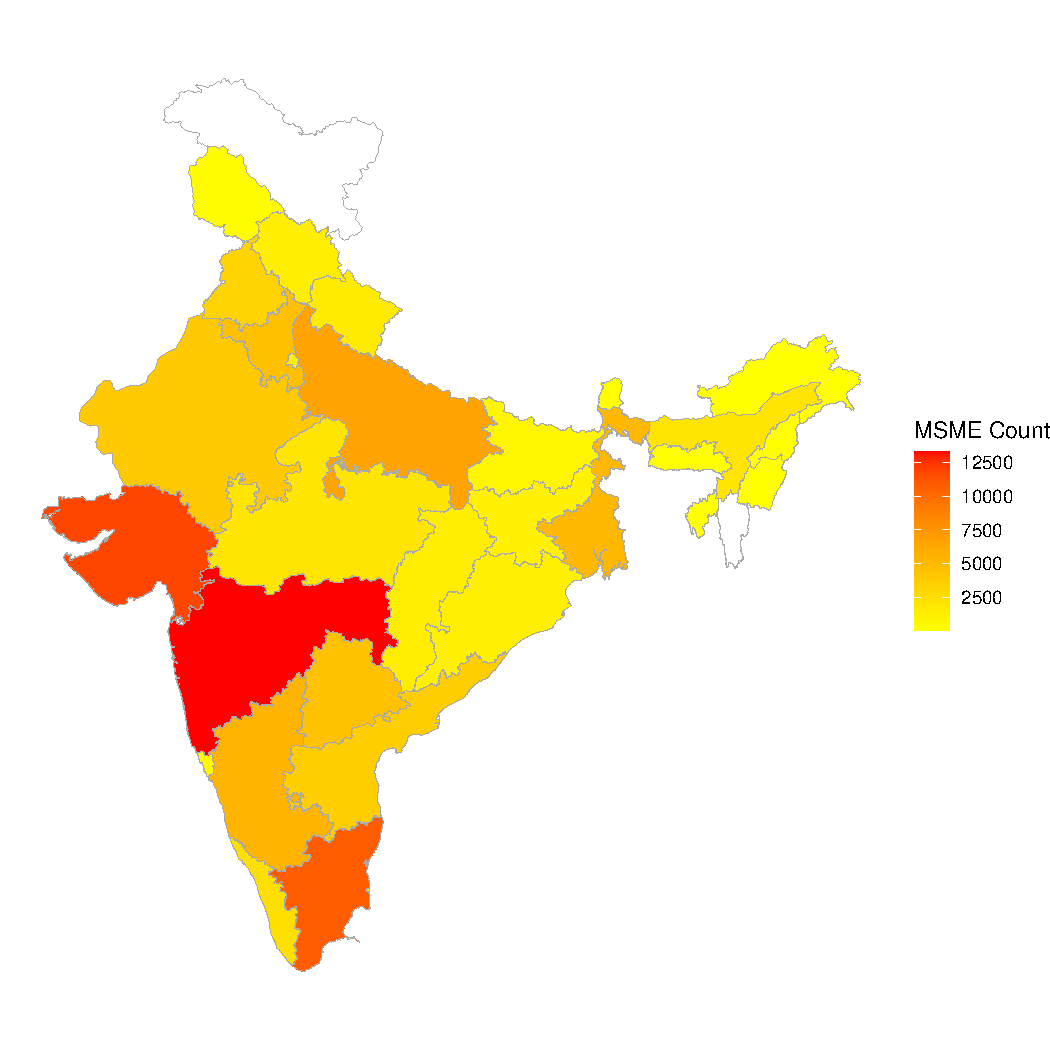
\includegraphics[width=\linewidth]{msme_plot.pdf}
        \caption{MSME in 2019}
        \label{fig:msme_plot}
    \end{minipage}
    \hfill
    \begin{minipage}[b]{0.45\textwidth}
        \centering
        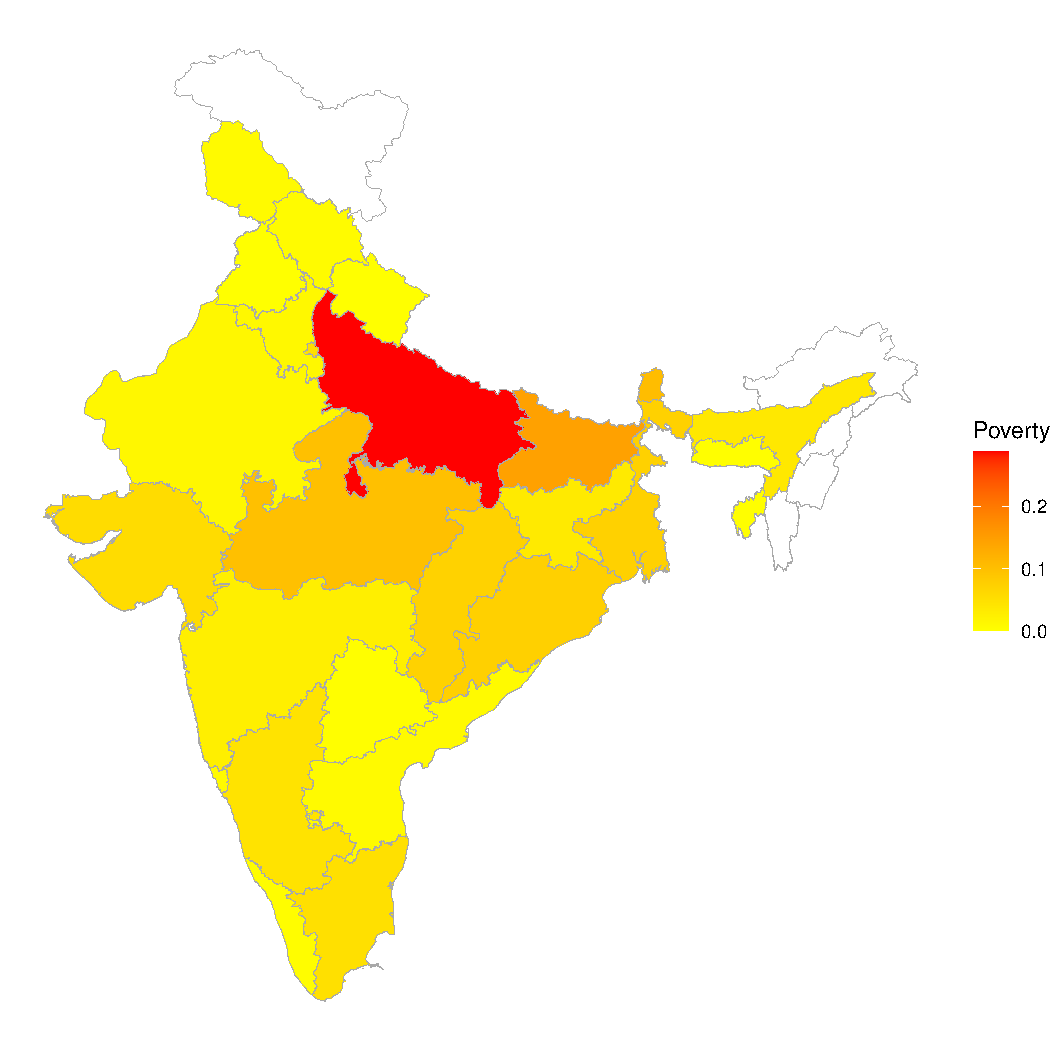
\includegraphics[width=0.95\linewidth]{poverty_plot.pdf}
        \caption{Poverty in 2019}
        \label{fig:poverty_plot}
    \end{minipage}
\end{figure}

\newpage
\newgeometry{left = 0.7cm, right = 0.7cm, bottom = 1.5cm, top = 1.5cm}

\section{Estimating the effect of MSME on poverty} \label{sec:models}
\paragraph{}  We used the Hausman test, which is a hypothesis test to determine whether to use fixed-effects or random-effects. As the Hausman test statistic has a p-value $\leq 0.05$ for all models, we choose fixed-effects model for this study. The data contain a panel of 25 states and 6 time periods. We perform separate estimations, for each poverty variable, one with poverty headcount ratio as the dependent variable, and a second with SMPCE as the dependent variable. Six estimations are done to find the empirical results: estimating the impact of MSMEs on poverty headcount ratio, estimating the impact of enterprise scale on poverty, and estimating the impact of groups\footnote{MSME are usually grouped into Small and medium (SME), and micro and small (MSE).} of MSME (MSE and SME) on poverty.

\vspace{0.3cm}
\noindent{\fontsize{14}{16}\selectfont\textbf{Models:}}
\vspace{0.3cm}

\text Since, the explanatory variables exhibit skewness, we apply a logarithmic transformation to them. This transformation corrects the skewness, and creates a more linear relationship between the variables. As a result, our estimations are better equipped to capture the true underlying connections between MSME and poverty. Additionally, to control for heterogeneity that are specific to different states and time periods, the models incorporate State fixed-effects and Time fixed-effects.

\text For model diagnostics, we use `Durbin-Watson' test for autocorrelation, `Breusch-Pagan' test for heteroscedasticity, and Variance Inflation Factor (VIF) for multicollinearity. The diagnostic tests show evidence of autocorrelation and heteroscedasticicy in the data, hence, we use robust standard errors, clustered at the state level. Robust standard errors are computed using Heteroscedasticity Consistent Covariance Matrix (HCCM) type HC3.\footnote{See \textcite{380055f1-819e-3149-a01c-cfab4e53c79f}}. \textcite{MACKINNON1985305} suggests that HC3 is suitable for small sample sizes and reduces the impact of leverages on the computation of standard errors. 

\begin{flalign}
    &{P_{it}} = \beta_0 + \beta_1\ln{MSME_{it}} + \beta_2\ln{SGDP_{it}} + \beta_3\ln{Yield_{it}} + \beta_4{Urban_{it}} + \beta_5\ln{Population_{it}} + \epsilon_{it} \label{1} && \\[0.2cm]
    &{SMPCE_{it}} = \beta_0 + \beta_1MSME_{it} + \beta_2SGDP_{it} + \beta_3Yield_{it} + \beta_4Urban_{it} + \beta_5{Population_{it}} + \epsilon_{it} \label{2} && \\[0.2cm]
    &P_{it} = \beta_0 + \beta_1\ln{Micro}_{it} + \beta_2\ln{Small}_{it} + \beta_3\ln{Medium}_{it} + \beta_4\ln{SGDP_{it}} + \beta_5\ln{Yield_{it}} + \beta_6Urban_{it} + \beta_7\ln{Population_{it}} + \epsilon_{it} \label{3} && \\[0.2cm]
    &{SMPCE_{it}} = \beta_0 + \beta_1{Micro}_{it} + \beta_2{Small}_{it} + \beta_3{Medium}_{it} + \beta_4SGDP_{it} + \beta_5Yield_{it} + \beta_6Urban_{it} + \beta_3{Population_{it}} + \epsilon_{it} && \label{4} \\[0.2cm]
    &{P_{it}} = \beta_0 + \beta_1\ln{MSE}_{it} + \beta_2\ln{Medium}_{it} + \beta_3\ln{SGDP_{it}} + \beta_4\ln{Yield_{it}} + \beta_5Urban_{it} + \beta_6\ln{Population_{it}} + \epsilon_{it} \label{5} \\[0.2cm]
    &{P_{it}} = \beta_0 + \beta_1\ln{SME}_{it} + \beta_2\ln{Micro}_{it} + \beta_3\ln{SGDP_{it}} + \beta_4\ln{Yield_{it}} + \beta_5Urban_{it} + \beta_6\ln{Population_{it}} + \epsilon_{it} \label{6} && 
\end{flalign}


\text In equation~\ref{1}, we explore the relationship between the poverty headcount and the natural log of MSME, alongside control variables, to assess the cumulative impact of MSME on poverty reduction. Equation~\ref{2} investigates how consumption levels are influenced by MSME, aiming to elucidate the combined effect of MSME on consumption of households. Equation~\ref{3} and ~\ref{4} are dedicated to examining the individual contributions of MSME (Micro, small, and medium as individual variables) to poverty alleviation and consumption, respectively. Finally, equations~\ref{5} and~\ref{6} focus on the grouped effects of MSME, analyzing their impact on poverty.

\newpage
\newgeometry{top = 1.2cm, bottom = 2 cm}

\section{Empirical results}
\begin{table}[htbp]
    \centering
    \smaller
    \caption{Regression Results}
\begin{tabular}{lcccccc}
    \toprule
    \toprule
     & (1) & (2) & (3) & (4) & (5) & (6) \\
    Term & \(P\) & \(SMPCE\) & \(P\) & \(SMPCE\) & \(P\) & \(P\) \\
    \midrule
    \textit{MSME} & $-16.337^{*}$ & $-0.060$ & & & & \\
                  & $(9.529)$ & $(0.058)$ & & & & \\
                   
    \textit{Micro} & & & $7.384$ & $0.037$ & & $6.657$ \\
                   & & & $(4.710)$ & $(0.340)$ & & $(4.570)$ \\
                   
    \textit{Small} & & & $-21.685^{***}$ & $-0.648$ & & \\
                   & & & $(7.644)$ & $(0.465)$ & & \\
                   
    \textit{Medium} & & & $-19.112^{**}$ & $0.417$ & $-22.836^{**}$ & \\
                    & & & $(8.121)$ & $(0.276)$ & $(9.033)$ & \\
                    
    \textit{MSE} & & & & & $-4.760$ &  \\
                 & & & & & $(8.199)$ &  \\
                 
    \textit{SME} & & & & & & $-37.647^{***}$ \\
                 & & & & & & $(10.2412)$\\
                      
    \textit{SGDP} & $-17.775$ & $0.004^{***}$ & $-17.542$ & $0.003^{*}$ & $-11.187$ & $-20.097$ \\
                  & $(19.167)$ & $(0.001)$ & $(14.547)$ & $(0.001)$ & $(17.761)$ & $(16.203)$ \\
                  
    \textit{Urban.} & $2.680^{**}$ & $-65.451^{*}$ & $2.723^{***}$ & $-50.812$ & $2.589^{**}$ & $2.795^{***}$ \\
                   & $(1.281)$ & $(38.667)$ & $(1.002)$ & $(40.534)$ & $(1.221)$ & $(1.044)$ \\
                   
    \textit{Yield}  & $12.810$ & $0.100$ & $8.924$ & $0.099$ & $11.493$ & $ 9.416$ \\
                    & $(9.042)$ & $(0.166)$ & $(8.031)$ & $(0.162)$ & $(8.486)$ &  $(8.103)$\\
    \textit{Population} & $223.283^{*}$ & $-0.000^{*}$ & $ 270.026^{**}$ & $-0.000$ & $259.609^{**}$ & $251.890^{**}$ \\
                        & ($131.256$) & ($0.000$) & ($108.222$) & ($0.000$) & ($126.023$) & ($107.417$) \\
    \bottomrule
    Obs & 137 & 137 & 137 & 137 & 137 & 137 \\
    $R^{2}$ & 0.17 & 0.075 & 0.17 & 0.09 & 0.22 & 0.24 \\
    F-stat & 4.151 & 1.664 & 4.151 & 1.488 &  4.7129 & 5.363 \\
    P-value & $\leq 0.001$ & $0.149$ & $\leq 0.001$ & $0.179$ & $\leq 0.001$ & $\leq 0.001$ \\
    \bottomrule
    \bottomrule
\end{tabular}
    \label{tab:results}
    \begin{tablenotes}[flushleft] 
        \smaller
        \item[*] ***: pvalue $\leq 0.01$, **: pvalue $\leq 0.05$, * : pvalue $\leq 0.1$ 
        \vspace{0.1cm}
        \item[**] Robust Standard errors are clustered at the state level and presented in parentheses.
        \item[***] Fixed effects are presented in table~\ref{tab:5} in ~\nameref{sec:appendix}.

    \end{tablenotes}
\end{table}

\text Results from equation~\ref{1} show that the number of MSME has a poverty-alleviating effect in India, 1\% increase in the count MSME reduce the poverty headcount\footnote{Where poverty headcount ranges from 0 to 1.} by 0.16 percentage points, however, from equation~\ref{2}, the influence of MSME on consumption is not statistically significant. Equation~\ref{3} reveals an impact of enterprise-scale: micro entrepreneurs, exhibit a positive correlation with the poverty headcount but the coefficient is statistically insignificant. In contrast, small and medium enterprises significantly contribute to poverty alleviation. From equation~\ref{3}, we infer that a 1\% increase in small enterprises reduces the poverty headcount by 0.21 percentage points, and 1\% increase in medium enterprises reduces poverty headcount by 0.19 percentage points. From equation~\ref{4}, micro, small, or medium enterprises seem to have no significant effect on consumption. The F statistic is deemed insignificant for consumption models (equation~\ref{2} and equation~\ref{4}, indicating that the explanatory variables collectively exert no substantial impact on consumption. When analysed in groups (equation~\ref{5} and \ref{6}), SMEs demonstrate a substantial effect in reducing poverty. From equation~\ref{6} we infer that 1\% increase in the number of SME will reduce poverty by 0.37 percentage points. From equation~\ref{6}, micro enterprises do not have a significant effect on poverty. From Equation~\ref{5} we note that MSE have no significant effect on poverty, and medium enterprises have a negative significant coefficient, which is in line with results from equation~\ref{3}.  
\text The coefficient for micro enterprises in table~\ref{tab:results} is positive, although insignificant.  A possible reason for micro enterprises not contributing to poverty alleviation could be their limited capital, as they inherently have the least financial resources. This lack of capital can lead to difficulties in expanding the business and may force these enterprises to use informal labour to save costs if it even employs people. \textcite{kanitkar1994entrepreneurs} finds in his sample that 32\% reported that their enterprises did not employ any person on a full time basis. The remaining 68\% entrepreneurs employed an average of 2.77 persons per enterprise. He concludes that the employment figures suggest that the enterprises had limited potential in providing employment to fellow villagers.
 \text Additionally, limited funds might mean using less advanced technology, resulting in lower productivity. Consequently, micro enterprises might offer lower wages than small and medium enterprises. Together, these factors suggest that micro enterprises could unintentionally worsen poverty due to these inherent limitations and inefficiencies. SME by definition have more capital than micro, thus can operate at a bigger scale, use better technologies, and employ more people, possibly at better wage rates. Thus, SME (individually, and grouped) have a poverty-alleviating effect. When micro enterprises expand, they evolve into small enterprises. This progression is accompanied by an enhancement in the enterprise's capabilities, which can have positive implications for both employment opportunities and wage levels within the enterprise.


\section{Limitations}
\paragraph{}
While this study provides us with further insights into the relationship between MSME and poverty, there are several limitations that need to be addressed. \textcite{somanchi2021missing} refutes the claim of CPHS being nationally representative and claims that it underrepresents women and young children, overrepresents well-educated households, and underrepresents the poor. \textcite{somanchi2021missing} also points out that CPHS has a major urban bias. CMIE's datacollection methodology is likely to provide a skewed sample since they start their sampling from each village's ``main street" or ``central circle" \parencite{somanchi2021missing}. \textcite{somanchi2021missing} suggests that Indian villages are spatially segregated spaces and better-off households tend to live closer to the village centre and marginalized groups like Scheduled Castes are often forced to the periphery. 
CMIE defends these claims in \textcite{economictimes2021}. \textcite{economictimes2021} claims that an average Indian village comprises about 300 households. ``In this systematic random sampling, every $n$th house is selected, where \textit{n} varies between 5 and 15, aiming for a sample size of 16. If \textit{n} is 5, 16 households would require at least 80 homes on the main street, a rare occurrence in village streets. Thus, accessing inner streets becomes necessary. For \textit{n} values of 10 and 15, the requirement for households increases to 160 and 240 respectively, making it even less likely to confine the sample to just the main street. Hence, including households from the outskirts is an inevitable part of the CPHS sampling method" \parencite{economictimes2021}.
Given the limitations of India's statistical system, including the absence of regular household surveys, we are compelled to rely on data from the CPHS, given its shortcomings. 

%\newpage
%\newgeometry{top=2cm, bottom = 2.2cm, left = 2.5cm, right = 2.5cm}
\paragraph{}
Since this study uses ASI data to compute MSME count in each state, it goes without saying that this study's findings are only limited to manufacturing MSME. \textcite{kanitkar1994entrepreneurs} finds that only 19\%  of rural micro enterprises in his sample are involved in manufacturing, while higher proportion of micro enterprises are involved in services. Even on a state level, \textcite{mor2020survival} finds 41\% of micro enterprises are involved in manufacturing in his sample in Haryana, while 46.8\% is involved in trading, and the rest in services. \textcite{manna2017status} points out that the number of unregistered MSME \footnote{MSME that aren't registered with District Industries Centre or Khadi and Village Industries Board or not included in the ASI frame} are much higher than the registered. Due to the lack of an alternative, we are impelled to use ASI data, despite its limitations.  

\text Another limitation of this study is that it uses consumption-based poverty headcount as the main unit of analysis. Amartya Sen in ``Equality of what?"  argues on using MDP over any resource-based poverty measure. Given the tight timeline and the intricate knowledge needed for other methods, We choose to use a resource-based poverty measure. The decision to employ a resource-based poverty measure is strategically motivated by a need for efficiency and pragmatism. This approach allows for a focused analysis within the available timeframe, ensuring that the study remains robust and actionable within its intended scope.

\section{Conclusion}

\paragraph{} This study computes the number of MSME and poverty headcount in India, and estimates the relation between these two variables. The study establishes that growth in the number of MSME contributes to poverty reduction in India. SME and MSE have different effects on poverty, SME have a significant alleviation effect, while MSE have no significant effect on poverty. It is concluded that individually, small and medium enterprises exhibit a significant negative impact on poverty, indicating their crucial role in poverty reduction efforts. Conversely, micro enterprises display a more complex relationship with poverty.
1\% increase in the number of MSME in a state reduces poverty by 0.16 percentage points. 1\% increase in the number of SME decrease poverty by 0.37 percentage points, 1\% in the number of small enterprises reduces poverty by 0.21 percentage points, and 1\% increase in the number of medium enterprises reduces poverty by 0.19 percentage points. This finding are consistent with those of \textcite{manzoor2019role}, who note the role of SMEs in increasing the incomes of India's lowest 20\%. Future research could beneficially explore the effects of labour absorption and the output of MSME as critical explanatory variables, rather than solely focusing on the count of MSME, for a deeper understanding of their role in poverty reduction. Instead of looking at just consumption-based poverty, MDP index can also be looked at for a more robust analysis.


\iffalse
\newpage
 \begin{figure}[htbp]
\centering
\caption*{Why Micro entrepreneurs may lead to increased poverty}
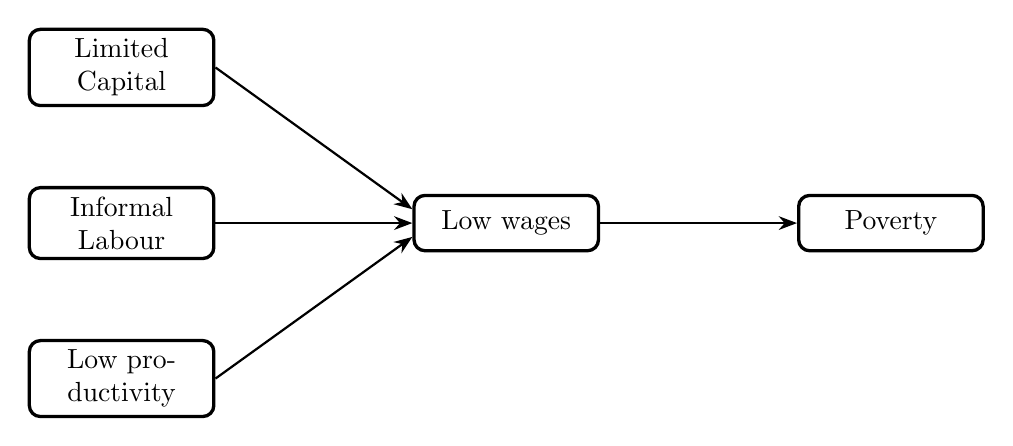
\begin{tikzpicture}[
    node distance=1cm and 2.5cm,
    auto,
    box/.style={rectangle, rounded corners, draw=black, very thick, text width=6em, minimum height=2em, text centered},
    line/.style={draw, thick, -Stealth}
    ]

    % Nodes
    \node (informal) [box] {Limited Capital};
    \node (economies) [box, below=of informal] {Informal Labour};
    \node (capital) [box, below=of economies] {Low productivity};
    \node (wages) [box, right=of economies] {Low wages};
    \node (poverty) [box, right=of wages] {Poverty};

    % Arrows
    \draw [line] (informal.east) -- ([yshift=5pt]wages.west);
    \draw [line] (economies.east) -- (wages.west);
    \draw [line] (capital.east) -- ([yshift=-5pt]wages.west);
    \draw [line] (wages) -- (poverty);
\end{tikzpicture}
\end{figure}
\fi
%\printbibliography

\newpage
\newgeometry{right = 1.8cm, left = 1.8cm, top = 2cm, bottom = 2cm}
\pagenumbering{roman}
\appendix 
\section{Appendix} \label{sec:appendix}
\subsection*{CPHS data collection }
\begin{table}[htbp]
    \centering
    \caption{Summary of Waves}
    \begin{tabular}{cccc}
        \toprule
        \textbf{Wave} & \textbf{Period} & \textbf{Unique Count} & \textbf{Total Observations (\%)} \\
        \midrule
        
        6 & May-Aug 2019 & 174,405 & 147,868 (84.78\%) \\
        5 & May-Aug 2018 & 172,365 & 149,160 (86.54\%) \\
        4 & May-Aug 2017 & 160,847 & 132,686 (82.49\%) \\
        3  & May-Aug 2016 & 159,778 & 132,399 (82.86\%) \\
        2  & May-Aug 2015 & 158,666 & 135,746 (85.55\%) \\

        1  & May-Aug 2014 & 160,705 & 140,692 (87.55\%) \\

        \hline
        \textbf{Unique count} & \textbf{All Waves} & \textbf{240,220} & \textbf{218,438 (90.93\%)} \\
        \textbf{Total observations} & \textbf{All Waves} & \textbf{5,098,616} & \textbf{3,940,643 (77.29\%)} \\
        \bottomrule
    \end{tabular}
\end{table}

\subsection*{Isolated effects of Micro, Small, Medium, SME and MSE}

\text In the section \nameref{sec:models}, we do not regress poverty variables against only Micro, Small, or Medium since in the real world all three coexist together, and cannot be isolated. The same logic applies to SME and MSE. However, for robustness, we run poverty variables against individual MSME in isolation. The same fixed-effects models as in section \ref{sec:models} are used for this exercise. 
\begin{equation}\label{7}
   {P_{it}} = \beta_0 + \beta_1\ln{Micro}_{it} + \beta_4\ln{SGDP_{it}} + \beta_5\ln{Yield_{it}} + \beta_6Urbanisation_{it}  + \beta_7\ln{Population_{it}}+ \epsilon_{it}
\end{equation}

\begin{equation}\label{8}
   {P_{it}} = \beta_0 + \beta_1\ln{Small}_{it} + \beta_4\ln{SGDP_{it}} + \beta_5\ln{Yield_{it}} + \beta_6Urbanisation_{it} + \beta_7\ln{Population_{it}} + \epsilon_{it}
\end{equation}

\begin{equation}\label{9}
   {P_{it}} = \beta_0+ \beta_1\ln{Medium}_{it} + \beta_4\ln{SGDP_{it}} + \beta_5\ln{Yield_{it}} + \beta_6Urbanisation_{it} + \beta_7\ln{Population_{it}} + \epsilon_{it}
\end{equation}

\begin{equation}\label{10}
P_{it} = \beta_0 + \beta_1\ln{{MSE}}_{it} + \beta_3\ln{SGDP_{it}} + \beta_4\ln{Yield_{it}} + \beta_5Urbanisation_{it} + \beta_6\ln{Population_{it}}+ \epsilon_{it}     
\end{equation}

\begin{equation}\label{11}
P_{it} = \beta_0 + \beta_1\ln{{SME}}_{it} + \beta_3\ln{SGDP_{it}} + \beta_4\ln{Yield_{it}} + \beta_5Urbanisation_{it} + \beta_6\ln{Population_{it}}+ \epsilon_{it}     
\end{equation}

\newpage
\begin{table}[htbp]
    \centering
    \smaller
    \caption{Isolated regression effects}
    \begin{threeparttable}
        \begin{tabular}{lccccc}
            \toprule
            \toprule
            & (1) & (2) & (3) & (4) & (5) \\
            Term & \(P\) & \(P\) & \(P\) & \(P\) & \(P\) \\
            \midrule
                           
            \textit{Micro} & $-2.739$ & $ $ & $ $ & $ $ & $ $ \\
                           & ($4.085$) & $ $ & $ $ & $ $ & $ $ \\
                           
            \textit{Small} & $ $ & $-23.870^{***}$ & $ $ & $ $ & $ $ \\
                           & $ $ & ($6.902$) & $ $ & $ $ & $ $ \\
                           
            \textit{Medium} & $ $ & $ $ & $-25.136^{***}$  & $ $ & $ $ \\
                            & $ $ & $ $ & ($9.469$)  & $ $ & $ $ \\
                            
            \textit{MSE} & $ $ & $ $ & $ $ & $-14.003^{*}$ & $ $ \\
                         & $ $ & $ $ & $ $ & ($7.798$) & $ $ \\
                         
            \textit{SME} & $ $ & $ $ & $ $ & $ $ & $-31.511^{***}$ \\
                         & $ $ & $ $ & $ $ & $ $ & ($9.984$) \\
                                  
            \textit{SGDP} & $-18.042$ & $-22.434$  & $-10.293$ & $-19.090$  & $-18.469$ \\
                          & ($21.130$) & ($16.341$) & ($ 11.915$)  & ($19.128$)  & ($16.484$) \\
                          
            \textit{Urban} & $2.642^{*}$ & $2.807^{***}$  & $ 2.559^{**}$ & $ 2.706^{**}$  & $ 2.775^{**}$ \\
                           & ($1.346$)  & ($1.019$)  & ($1.229$)  & ($1.249$)  & ($1.064$)  \\
                           
            \textit{Yield}  & $12.266$  & $11.649$  & $10.872$  & $13.098$ & $11.469$  \\
                            & ($ 8.981$)  & ($8.861$)  & ($8.441$)  & ($9.113$)  & ($ 8.610$)  \\
            \textit{Population} & $217.702$  & $236.989^{**}$ &  $262.007^{**}$&$222.979^{*}$ & $245.286^{**}$\\
                                & $(136.989)$ & $(108.498)$ & ($128.780$) &  ($128.852$) &  ($109.835$)\\
            \bottomrule
            Obs & 137 & 137 & 137 & 137 & 137 \\
            $R^{2}$ & 0.14 & 0.21  & 0.21 & 0.17  & 0.23  \\
            F-stat & 3.40     &  5.722  & 5.62  & 4.13  & 6.101  \\
            P-value & $< 0.001$ & $< 0.001$ & $< 0.001$ & $< 0.001$ & $< 0.001$ \\
            \bottomrule
            \bottomrule
        \end{tabular}
        \begin{tablenotes}[flushleft] 
            \smaller
            \item ***: p-value $\leq 0.01$, **: p-value $\leq 0.05$, *: p-value $\leq 0.1$
            \vspace{0.1cm}
            \item Robust Standard errors are clustered at the state level and presented in parentheses.
        \end{tablenotes}
    \end{threeparttable}
    \label{tab:results_extended}
\end{table}


\text In isolation, micro entrepreneurs seem to have no significant effect on poverty headcount, while small and medium entrepreneurs have significant poverty alleviation effects. This is in line with results from equation~\ref{2} in table~\ref{tab:results}. In isolation MSE have poverty alleviating effects, this is contrary to results from equation~\ref{4} in table~\ref{tab:results}. In isolation, SME have poverty alleviating effects, which is in line with equation~\ref{4} in table~\ref{tab:results}.

\newpage
\subsection*{Fixed Effects}
\begin{table}[htbp]
    \centering
    \caption{Coefficients of state fixed-effects}
    \label{tab:5}
    \begin{tabular}{lrrrrrrr}
    \toprule
    \toprule
    State & Equation ~\ref{1} & Equation ~\ref{2} & Equation ~\ref{3} & Equation ~\ref{4} & Equation ~\ref{5} & Equation ~\ref{6} \\
    \midrule
    Andhra Pradesh & -3796 & 6651 & -4493 & 6069 & -4436 & -4139 \\
    Assam & -3665 & 4376 & -4365 & 4519 & -4316 & -4011 \\
    Bihar & -3951 & 8650 & -4735 & 8318 & -4660 & -4355 \\
    Chhattisgarh & -3633 & 4058 & -4327 & 3834 & -4272 & -3980 \\
    Delhi & -3749 & 8820 & -4444 & 7848 & -4395 & -4098 \\
    Goa & -3129 & 7554 & -3701 & 6906 & -3675 & -3405 \\
    Gujarat & -3853 & 8511 & -4543 & 8679 & -4495 & -4187 \\
    Haryana & -3672 & 5795 & -4335 & 5657 & -4296 & -3993 \\
    Himachal Pradesh & -3307 & 2805 & -3925 & 2867 & -3893 & -3602 \\
    Jharkhand & -3707 & 4745 & -4418 & 4494 & -4359 & -4066 \\
    Karnataka & -3842 & 8169 & -4550 & 8095 & -4497 & -4192 \\
    Kerala & -3790 & 8231 & -4488 & 7758 & -4436 & -4139 \\
    Madhya Pradesh & -3877 & 7678 & -4613 & 7333 & -4547 & -4249 \\
    Maharashtra & -3983 & 12624 & -4702 & 12753 & -4646 & -4335 \\
    Meghalaya & -3239 & 2957 & -3881 & 2751 & -3841 & -3562 \\
    Odisha & -3706 & 4375 & -4430 & 4239 & -4369 & -4073 \\
    Puducherry & -3119 & 6254 & -3691 & 5425 & -3660 & -3398 \\
    Punjab & -3699 & 6479 & -4371 & 6252 & -4326 & -4027 \\
    Rajasthan & -3849 & 7771 & -4569 & 7744 & -4511 & -4207 \\
    Sikkim & -2946 & 3377 & -3528 & 3109 & -3502 & -3234 \\
    Tamil Nadu & -3898 & 9594 & -4594 & 9307 & -4543 & -4237 \\
    Tripura & -3339 & 4056 & -4028 & 3661 & -3975 & -3695 \\
    Uttar Pradesh & -4082 & 16281 & -4846 & 16146 & -4776 & -4467 \\
    Uttarakhand & -3457 & 4881 & -4087 & 4678 & -4055 & -3759 \\
    West Bengal & -3925 & 9258 & -4652 & 9345 & -4593 & -4287 \\
    \midrule
    Average & -3649 &  6958 & -4333 & 6711 & -4283 & -3988 \\
    \bottomrule
    \bottomrule
    \end{tabular}
\end{table}

\newpage
\restoregeometry
\printbibliography
\end{document}
